\section{HDSDP Software}\label{sec5}

{{\texttt{HDSDP}}} is written in \text{{\ttfamily{ANSI C}}} and provides a
self-contained user interface. While {{\texttt{DSDP}}} serves as a sub-routine library, 
{{\texttt{HDSDP}}} is designed to be a stand-alone SDP solver and re-written to accommodate the 
new computational tricks and third-party packages.  After the user inputs the data and invokes the
optimization routine, {{\texttt{HDSDP}}} goes through several modules
including input check, pre-solving, two-phase optimization, solution recovery
and post-solving. The modules are implemented independently and are
sequentially organized in a pipeline by {{\texttt{HDSDP}}}.

\subsection{Pre-solver}

One important feature of {{\texttt{HDSDP}}} is a special pre-solving module
 designed for SDPs. It inherits strategies from
{{\texttt{DSDP5.8}}} and adds new tricks to work jointly with the
optimization module.\\

When the pre-solver is invoked, it first goes through the problem data
$\left\{ \mathbf{A}_i \right\}$ two rounds to detect the possible low-rank structure.
The first round uses Gaussian elimination for rank-one structure and the
second round applies eigenvalue decomposition from \text{{\ttfamily{Lapack}}}. Two
exceptions are when the data matrix is too dense or sparse. If a matrix looks
too dense to be decomposed efficiently, it is skipped and marked as full-rank;
if it has very few entries, an elegant solution from {{\texttt{DSDP5.8}}} is
applied: {\textbf{1)}} a permutation gathers the non-zeros to a much smaller
dense block. {\textbf{2)}} dense eigen routines from \text{{\ttfamily{Lapack}}}
applies. {\textbf{3)}} the inverse permutation recovers the decomposition.\\

After detecting the hidden low-rank structures, the pre-solver moves on to
the analysis of the Schur matrix $\mathbf{M}$: {\textbf{1)}}. the sparsity and rank
information of the matrices are collected. {\textbf{2)}}. a permutation of
$\left\{ \mathbf{A}_i \right\}$ is generated in descending order of sparsity.
{\textbf{3)}}. for each row of $\mathbf{M}$, the flops using each of {\textbf{M1}}
to {\textbf{M5}} technique is computed and the cheapest technique is
recorded. The recorded techniques reduces the flops to set up $\mathbf{M}$ and
accelerates the convergence.\\

Last the pre-solver scales the coefficients and goes on to detect the
following structures. {\textbf{1)}}. Implied trace: constraints implying
$\ensuremath{\operatorname{tr}} \left( \mathbf{X} \right) = \theta$. {\textbf{2)}}. Implied dual bound:
constraints implying $\mathbf{l} \leq \mathbf{y} \leq \mathbf{u}$. {\textbf{3)}}. Empty
primal interior: constraints implying $\ensuremath{\operatorname{tr}} \left( \mathbf{X} \mathbf{a} \mathbf{a}^{\top}
\right) \approx 0$. {\textbf{4)}}. Empty dual interior: constraints implying
$\mathbf{A}^{\top} \mathbf{y} = \mathbf{C}$. {\textbf{5)}}. Feasibility problem. $\mathbf{C} = \textbf{0}$. For each
of the cases above the solver adjusts its internal strategies to enhance the
numerical stability and convergence.

\subsection{Two-phase Optimization}

{{\texttt{HDSDP}}} implements two phase-algorithm which integrates HSD
embedding (\text{{\ttfamily{Phase A}}}) and dual-scaling (\text{{\ttfamily{Phase B}}}). \
\text{{\ttfamily{Phase A}}} targets feasibility certificate and numerical stability,
while \text{{\ttfamily{Phase B}}} aims to efficiently drive a dual-feasible solution to
optimality using potential function.

\begin{figure}[h]
\centering
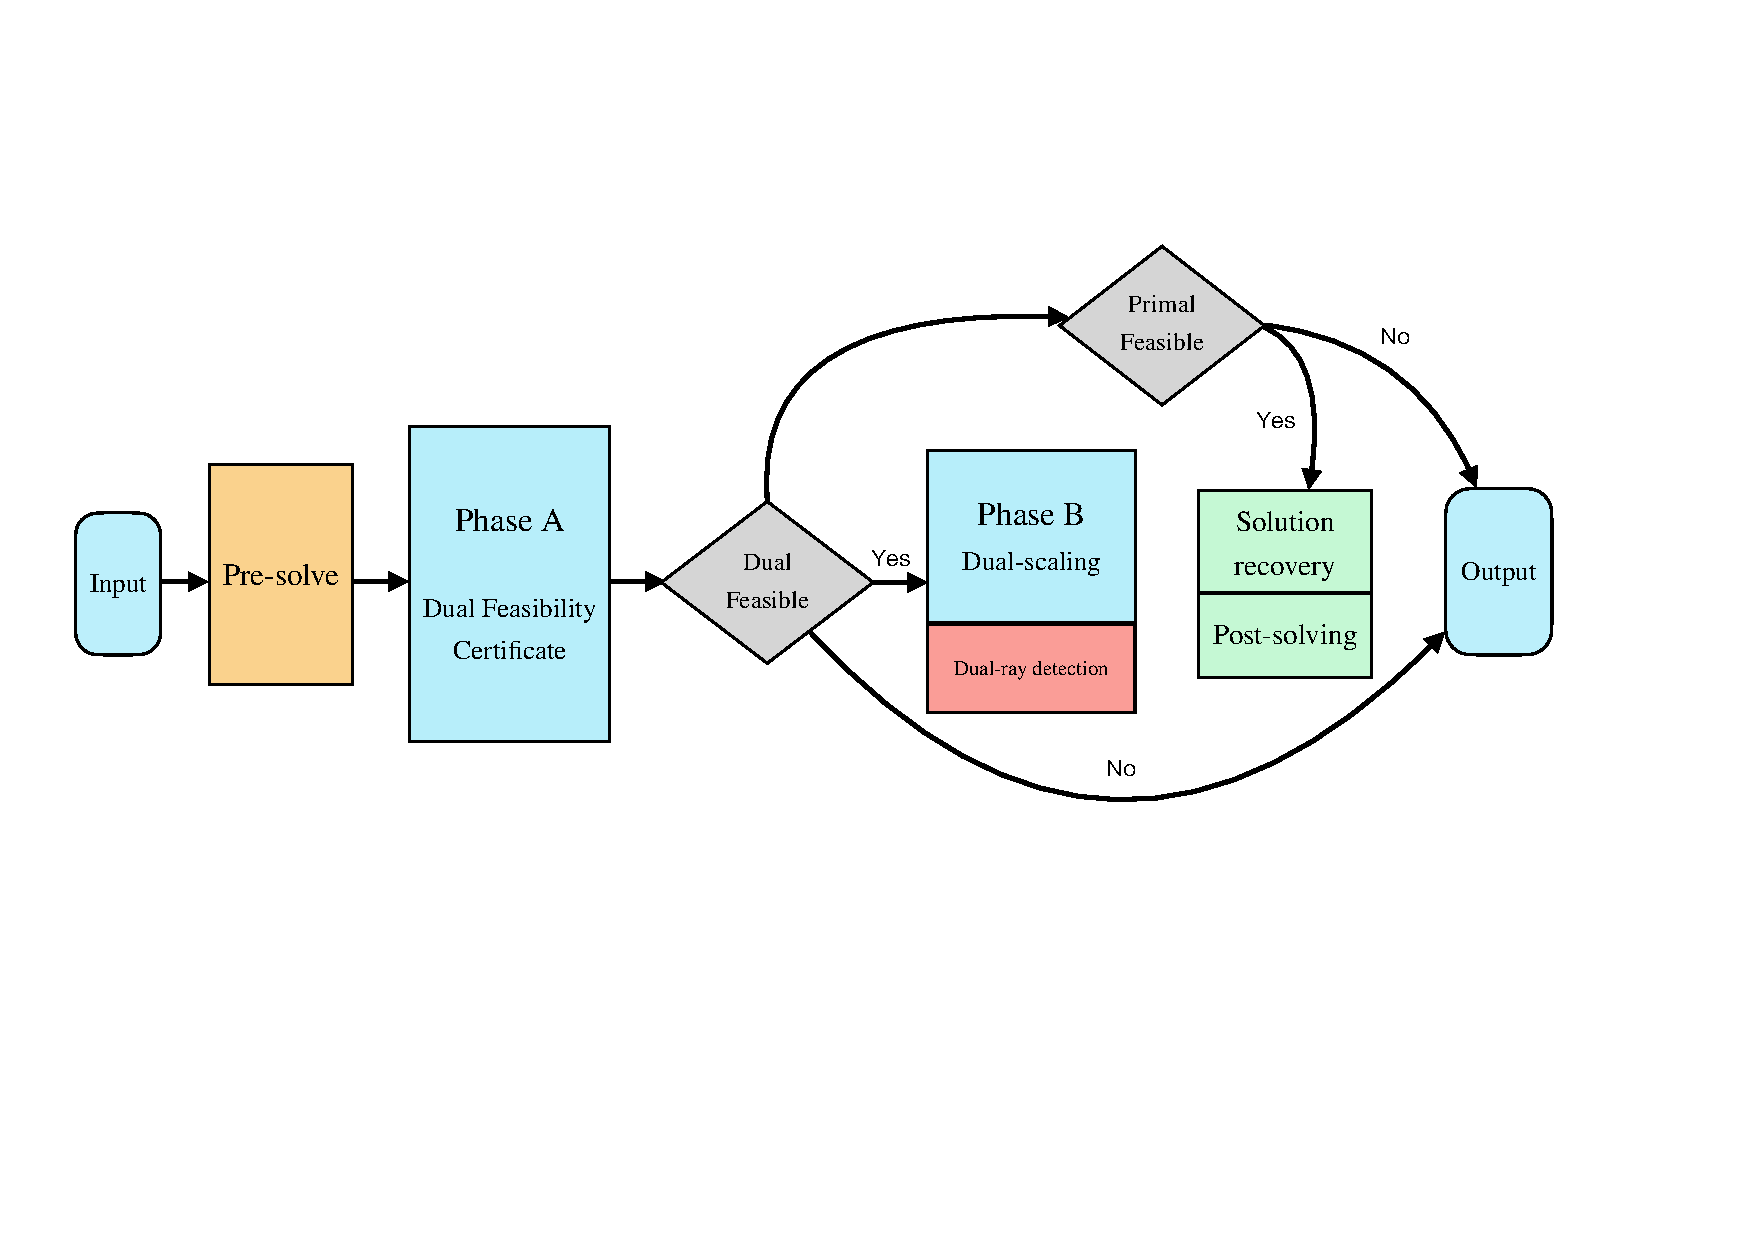
\includegraphics[scale=0.5]{fig.pdf}
  \caption{Pipeline of {{\texttt{HDSDP}}}}
\end{figure}

\

In a word, the two phases share the same backend computation routines but are
associated with different goals and strategies. {{\texttt{HDSDP}}} decides
which strategy to use based on the solution behavior.

\subsection{Iteration Monitor}

To help the users capture the progress of the solver, {{\texttt{HDSDP}}}
prints related information to the screen at different stages of optimization. 
\begin{lstlisting}
--------------------------------------------------------------------------------------
| Start presolving 
| - XXX completes in 0.001 seconds 
| - Matrix statistics ready in 0.000 seconds 
|    Schur Re-ordering: M1: 0  M2: 3000  M3: 0  M4: 1  M5: 0 
| - Special structures found 
|    tr(X) = 3.00e+03 : Bound of X fixed 
| Presolve Ends. Elapsed Time: 0.371 seconds 
--------------------------------------------------------------------------------------
\end{lstlisting}
While pre-solving, {{\texttt{HDSDP}}} prints time statistics when certain operation
is done. Specially, the row
\begin{tmcode}
      Schur Re-ordering: M1: 0  M2: 3000  M3: 0  M4: 1  M5: 0
\end{tmcode}
indicates how many times each Schur complement technique is applied and if
special SDP structures are detected, they are also printed to the screen.
\begin{tmcode}
      tr(X) = 3.00e+03 : Bound of X fixed.
\end{tmcode}
When the pre-solving ends, {{\texttt{HDSDP}}} prints matrix statistics
including type and sum of norm. Also, the solver internally adjusts its parameters
based on the collected information and display them to the user. 

\begin{lstlisting}
--------------------------------------------------------------------------------------
| Matrix statistics [Including C]: 
--------------------------------------------------------------------------------------
|     Zero |   Sparse |    Dense |   Rank-1 |      |A|    |      |b|    |      |C|     
--------------------------------------------|-----------------------------------------
|        0 |        1 |        0 |     3000 |  3.0000e+03 |  3.0000e+03 |  1.2000e+04 
--------------------------------------------------------------------------------------
| Parameter Summary: 
--------------------------------------------------------------------------------------
| Rhon [1.0, 10.0]: 5 
| Golden linesearch \{0, 1\}: 0 
| Primal relaxation penalty (0.0, inf): 1e+07 
| Time limit (0.0, inf): 15000 
| Corrector A: 4  Corrector B: 0 
--------------------------------------------------------------------------------------
| DSDP is initialized with Ry = -1.225e+05 * I                                                     
| DSDP Phase A starts. Eliminating dual infeasibility                                              
--------------------------------------------------------------------------------------
\end{lstlisting}

After pre-solving, {{\texttt{HDSDP}}} enters optimization, invokes HSD embedding (\text{{\ttfamily{Phase A}}}), and prints logs.

\begin{lstlisting}
--------------------------------------------------------------------------------------
| Iter |     pObj |     dObj |     dInf |     k/t |      mu |   step |   Pnorm |   E |
--------------------------------------------------------------------------------------
|    1 |  1.0e+05 |  0.0e+00 | 6.71e+06 | 1.0e+00 | 4.0e+04 |   0.00 | 1.0e+20 |     |
|    2 |  2.4e+08 | -7.3e+08 | 0.00e+00 | 1.0e+00 | 3.8e+04 |   1.00 | 1.1e+02 |   * |
--------------------------------------------------------------------------------------	
\end{lstlisting}


\begin{table}[h]
\centering
  \begin{tabular}{r|l}
        \hline
    \text{{\ttfamily{Iter}}} & the iteration number\\
    \text{{\ttfamily{pObj}}} & the primal objective bound\\
    \text{{\ttfamily{dObj}}} & the dual objective \\
    \text{{\ttfamily{k/t}}} & $\kappa / \tau$ from the embedding\\
    \text{{\ttfamily{mu}}} & the current barrier parameter\\
    \text{{\ttfamily{step}}} & stepsize $\alpha$ taken\\
    \text{{\ttfamily{Pnorm}}} & the proximity to the central path\\
    \text{{\ttfamily{E}}} & event monitor\\
    \hline    
  \end{tabular}
  \caption{Iteration monitor of Phase \text{{\ttfamily{A}}}}
\end{table}

When \text{{\ttfamily{Phase A}}} finds a dual-feasible solution, {{\texttt{HDSDP}}}
collection the solution statistics to adjust the parameters for
dual-scaling in \text{{\ttfamily{Phase B}}}, prints related information and performs re-start.

\begin{lstlisting}
--------------------------------------------------------------------------------------
| DSDP Phase A ends with status: DSDP_PRIMAL_DUAL_FEASIBLE                                         
| Elapsed Time: 0.535 seconds                                                                   
--------------------------------------------------------------------------------------
| DSDP Phase A certificates primal-dual feasibility                                                
| Primal relaxation penalty is set to  2.449e+06 
| Perturbing dual iterations by  0.000e+00 
| DSDP Phase B starts. Restarting dual-scaling                                                     
| Heuristic start: mu:  2.177e+04 pObj:  2.450e+08  dObj: -7.346e+08                              
--------------------------------------------------------------------------------------
\end{lstlisting}	

The log from \text{{\ttfamily{Phase B}}} is similar to \text{{\ttfamily{Phase A}}} but
\text{{\ttfamily{dInf}}} is now replaced by \text{{\ttfamily{pInf}}} to characterize primal
infeasibility. Also, \text{{\ttfamily{k/t}}} is dropped from log since the embedding
is not applied.

\begin{lstlisting}
--------------------------------------------------------------------------------------
| Iter |        pObj |        dObj |       pInf |       mu |   step |    Pnorm |   E |
--------------------------------------------------------------------------------------
|    1 |  2.4500e+08 | -7.3462e+08 |  3.001e+03 | 2.18e+04 |   1.00 |  1.1e+02 |     |
|    2 |  2.4500e+08 | -3.6742e+07 |  3.001e+03 | 2.18e+04 |   0.09 |  5.6e+02 |     |
|    3 |  1.3061e+08 | -1.8487e+06 |  8.915e-03 | 3.72e+03 |   0.41 |  1.3e+02 |   P |
...
|   14 | -1.1997e+04 | -1.2000e+04 |  9.510e-11 | 4.66e-06 |   0.00 |  9.4e+00 |   P |
|   15 | -1.1999e+04 | -1.2000e+04 |  1.902e-12 | 9.32e-07 |   0.02 |  5.1e+01 |   F |
--------------------------------------------------------------------------------------
\end{lstlisting}

When \text{{\ttfamily{Phase B}}} converges, the solver extracts the solution status,
recovers primal feasible solution (if available) and briefly prints solution
and time statistics.

\begin{lstlisting}
--------------------------------------------------------------------------------------
| DSDP Phase B ends with status: DSDP_INTERNAL_ERROR                                               
| Elapsed Time: 5.960 seconds                                                                   
--------------------------------------------------------------------------------------
| DSDP Ends.                                                                                        
--------------------------------------------------------------------------------------
| Primal solution is extracted.                                                                    
| Final pObj: -1.19993e+04   dObj: -1.20000e+04 
--------------------------------------------------------------------------------------
| DSDP Time Summary: 
--------------------------------------------------------------------------------------
|           Event |    Time(s) | 
--------------------------------------------------------------------------------------
|        Presolve |      0.371 | 
|  Phase A (iter) |      0.535 | (2) 
|  Phase B (iter) |      5.960 | (15) 
|           Get X |      0.809 | 
|       Postsolve |      0.000 | 
|             All |      7.675 | (17) 
--------------------------------------------------------------------------------------
\end{lstlisting}

Compared to other IPM solvers, {{\texttt{HDSDP}}} tends to display more information so that the users better 
understand structures and features of the SDP instance. We believe that knowledge of
the problem structure would assist the users when customzing the solver for their applications.
